\documentclass{article}

\usepackage{float}
\usepackage{graphicx}
\usepackage{algorithm}
\usepackage{longtable}
\usepackage[utf8]{inputenc}
\usepackage[noend]{algpseudocode}

\title{Algoritmos - Lab4}
\author{Santiago Álvarez Sepúlveda }
\date{Octubre 15 2018}

\begin{document}

\maketitle

\section{Complete the Following Table}

\begin{longtable}[H]{|p{2.5cm}|p{2cm}|p{2cm}|p{2cm}|p{2cm}|}
\hline
\textbf{Algorithm} & \textbf{Worst case time complexity} & \textbf{Best case time complexity} & \textbf{Average case time complexity} & \textbf{Space complexity} \\ \hline
The simplest primality by trial division & $O(\sqrt{n})$ & $\Omega(1)$ & $\theta(\sqrt{n})$ & $O(1)$ \\ \hline
Binary Search & $O(n)$ & $\Omega(1)$ & $\theta(n)$ & $O(1)$ \\ \hline
Max or Min of Unsorted Array & $O(n)$ & $\Omega(n)$ & $\theta(n)$ & $O(1)$ \\ \hline
Kadane's algorithm & $O(n)$ & $\Omega(n)$ & $\theta(n)$ & $O(n)$ \\ \hline
Sieve of Eratosthenes  & $O(nlog(logn))$ & $\Omega(n)$ & $\theta(nlog(logn))$ & $O(n)$ \\ \hline
Merge Sort & $O(nlog(n))$ & $\Omega(nlog(n))$ & $\theta(nlog(n))$ & $O(n)$ \\ \hline
Heap Sort & $O(nlog(n))$ & $\Omega(nlog(n))$ & $\theta(nlog(n))$ & $O(1)$ \\ \hline
Quick Sort  & $O(n^2)$ & $\Omega(nlog(n))$ & $\theta(nlog(n))$ & $O(log(n))$ \\ \hline
Tim Sort & $O(nlog(n))$ & $\Omega(n)$ & $\theta(nlog(n))$ & $O(n)$ \\ \hline
Divide and conquer (Convex Hull) & $O(nlog(n))$ & $\Omega(nlog(n))$ & $\theta(nlog(n))$ & $O(n)$ \\ \hline
Insertion Sort & $O(n^2)$ & $\Omega(n)$ & $\theta(n^2)$ & $O(1)$ \\ \hline
Dijkstra's algorithm & $O(E log(V))$ & $\Omega(O(E log(V))$ & $\theta(O(E log(V))$ & $O(E+V)$ \\ \hline
Naive Matrix Multiplication & $O(2^{3n})$ & $\Omega(2^{3n})$ & $\theta(2^{3n})$ & $O(n)$ \\ \hline
Floyd–Warshall algorithm & $O(n^3)$ & $\Omega(n^3)$ & $\theta(n^3)$ & $O(n^3)$ \\ \hline
Naive Matrix Inversion & $O(n^3)$ & $\Omega(n^3)$ & $\theta(n^3)$ & $O(n)$ \\ \hline
Calculate the permutations of n distinct elements without repetitions & $O(n^2 n!)$ & $\Omega(n^2 n!)$ & $\theta(n^2 n!)$ & $O(1)$ \\ \hline
Calculate the permutations of n distinct elements with repetitions & $O(n^3)$ & $\Omega(n^3)$ & $\theta(n^3)$ & $O(1)$ \\ \hline
\end{longtable}


\section{Cormen, Leiserson, Rivest and Stein}

\subsection{Exercise 1.2-2}
Suppose we are comparing implementations of insertion sort and merge sort on the
same machine.  For inputs of size $n$, insertion sort runs in $8n^2$ steps, while merge sort runs in $64nlg(n)$ steps.  For which values of $n$ does insertion sort beat merge sort?

Sean $f(n) = 8n^2$ y $g(n) = 64nlg(n)$ las complejidades de los algoritmos de Insertion Sort y Merge Sort respectivamente, se pide encontrar el intervalo del parámetro $n$ para el cuál se cumple $f(n) < g(n)$.

\begin{figure}[H]
  \centering
  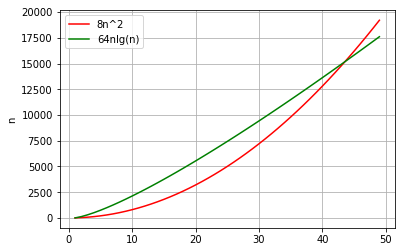
\includegraphics[width=\textwidth]{./img/CLRS_1_1}
  \caption{Visualización de cada función a analizar.}
  \label{fig:CLRS_1_1}
\end{figure}

por medio de un método numérico se halla una solución aproximada para valores enteros de $n$.

\begin{figure}[H]
  \centering
  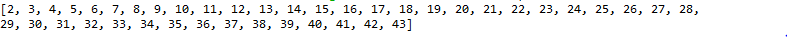
\includegraphics[width=\textwidth]{./img/CLRS_1_2}
  \caption{Resultados del método numérico (Hasta $N = 10^4$).}
  \label{fig:CLRS_1_2}
\end{figure}

Como se observa en la anterior figura, se tiene que el algoritmo de Insertion Sort será más rápido que el de Merge sorte para arreglos de tamaño $n = [2, 43]$.

\subsection{Excercise 1.2-3}
What is the smallest value of $n$ such that an algorithm whose running time is $100n^2$ runs faster than an algorithm whose running time is $2^n$ on the same machine?

Sean $f(n) = 100n^2$ y $g(n) = 2^n$ las complejidades de los algoritmos a analizar, se pide encontrar el menor $n$ para el cuál se cumple $f(n) < g(n)$.

\begin{figure}[H]
  \centering
  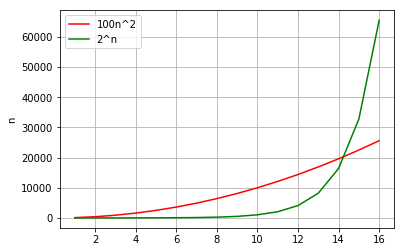
\includegraphics[width=\textwidth]{./img/CLRS_2_1}
  \caption{Método gráfico para hallar el menor $n$.}
  \label{fig:CLRS_2_1}
\end{figure}

por medio de un método numérico se halla una solución aproximada para valores enteros de $n$.

el menor entero que cumple esta condición es $n = 15$.

\subsection{Problem 1-1}
For each function $f(n)$ and time $t$ in the following table, determine the largest size $n$ of a problem that can be solved in time $t$, assuming that the algorithm to solve the problem takes $f(n)$ microseconds and nanoseconds.
Solve from 1 microsecond ($10^{-6}$ s) for step to for 1 nanoseconds ($10^{-9}$ s) for step.

Para resolver de forma general este problema, se ha identificado la solución del problema de la siguiente manera. Ya que $f(n)$ representa el tiempo de ejecución, en alguna escala de tiempo (micro o nano segundos), podemos entonces escribirlo de la siguiente manera:

$$f(n) = \alpha_t t$$

Donde $\alpha_t$ es un factor de conversión específico para transformar el tiempo de ejecución a micro o nano segundos.

Si existe una función inversa de $f(n)$, es decir $f^{-1}(n)$, esta función inversa nos relacionará el número de pasos realizados por el algoritmo, según el tiempo en micro o nano segundos que estuvo en ejecución.

$$n = f^{-1}(\alpha_t t)$$

Ya que en algunos casos no existe una función inversa (analítica) de la función $f(n)$, se resuelven estos casos por medio de métodos numéricos que permiten estimar iterativamente el valor de $n$ para un $\alpha_t t$ dado.

Se tiene la siguiente lista de factores de conversión $\alpha_t$:

\begin{longtable}[H]{|p{2.5cm}|p{2.5cm}|}
  \hline
  $\alpha_t$ & microsegundos \\ \hline
  $\alpha_{sec}$ & $1*10^6$ \\ \hline
  $\alpha_{min}$ & $6*10^7$ \\ \hline
  $\alpha_{hour}$ & $3.6*10^9$ \\ \hline
  $\alpha_{day}$ & $8.64*10^{10}$ \\ \hline
  $\alpha_{month}$ & $2.6784*10^{12}$ \\ \hline
  $\alpha_{year}$ & $3.15778*10^{13}$ \\ \hline
  $\alpha_{cent}$ & $3.15778*10^{15}$ \\ \hline
\end{longtable}

Las cantidades de estos factores de conversión, en unidades de nanosegundos son $10^3$ veces más grandes que los de microsegundos. Se consideraron para la anterior tabla el mes de $31$ días, un año como $365.25$ días y un siglo como $100$ de los años supuestos para considerar los años bisciestos.

\begin{longtable}[H]{|p{1.5cm}|p{1.5cm}|p{1.5cm}|p{1.5cm}|p{1.5cm}|p{1.5cm}|p{1.5cm}|p{1.5cm}|}
\hline
$f(n)$ & \textbf{1 Second} & \textbf{1 Minute} & \textbf{1 Hour} & \textbf{1 Day} & \textbf{1 Month} & \textbf{1 Year} & \textbf{1 Century} \\ \hline

 $lg(n)$ & $2^{\alpha_{sec}}$ & $2^{\alpha_{min}}$ & $2^{\alpha_{hour}}$ & $2^{\alpha_{day}}$ & $2^{\alpha_{month}}$ & $2^{\alpha_{year}}$ & $2^{\alpha_{cent}}$ \\ \hline
 
 $\sqrt(n)$ & $1*10^{12}$ & $3.6*10^{15}$ & $1.296*10^{19}$ & $7.465*10^{21}$ & $7.1738*10^{24}$ & $9.9588*10^{26}$ & $9.9588*10^{30}$ \\ \hline
 
 $n$ & $1*10^6$ & $6*10^7$ & $3.6*10^9$ & $8.64*10^{10}$ & $2.6784*10^{12}$ & $3.15778*10^{13}$ & $3.15778*10^{15}$ \\ \hline
 
 $n lg(n)$ & $6.2746*10^{4}$ & $2.801418*10^{6}$ & $1.333781*10^{8}$ & $2.755148*10^{9}$ & $7.417300*10^{10}$ & $7.981610*10^{11}$ & $1.154070*10^{14}$ \\ \hline
 
 $n^2$ & $1*10^{3}$ & $7.746*10^{3}$ & $6*10^{4}$ & $2.9394*10^{5}$ & $1.6366*10^{6}$ & $5.6176*10^{6}$ & $5.6176*10^{7}$ \\ \hline
 
 $n^3$ & $1*10^2{}$ & $3.91*10^{2}$ & $1.532*10^{3}$ & $4.42*10^{3}$ & $1.3888*10^{4}$ & $3.1601*10^{4}$ & $1.4668*10^{5}$ \\ \hline
 
 $2n$ & $5*10^5$ & $3*10^7$ & $1.8*10^9$ & $4.32*10^{10}$ & $1.3392*10^{12}$ & $1.5779*10^{13}$ & $1.5779*10^{15}$ \\ \hline
 
 $n!$ & $10$ & $12$ & $13$ & $14$ & $16$ & $17$ & $18$ \\ \hline
\end{longtable}

\begin{longtable}[H]{|p{1.5cm}|p{1.5cm}|p{1.5cm}|p{1.5cm}|p{1.5cm}|p{1.5cm}|p{1.5cm}|p{1.5cm}|}
\hline
$f(n)$ & \textbf{1 Second} & \textbf{1 Minute} & \textbf{1 Hour} & \textbf{1 Day} & \textbf{1 Month} & \textbf{1 Year} & \textbf{1 Century} \\ \hline

 $lg(n)$ & $2^{\alpha_{sec}}$ & $2^{\alpha_{min}}$ & $2^{\alpha_{hour}}$ & $2^{\alpha_{day}}$ & $2^{\alpha_{month}}$ & $2^{\alpha_{year}}$ & $2^{\alpha_{cent}}$ \\ \hline
 
 $\sqrt(n)$ & $1*10^{18}$ & $3.6*10^{21}$ & $1.296*10^{25}$ & $7.465*10^{27}$ & $7.1738*10^{31}$ & $9.9588*10^{32}$ & $9.9588*10^{36}$ \\ \hline
 
 $n$ & $1*10^9$ & $6*10^{10}$ & $3.6*10^{12}$ & $8.64*10^{13}$ & $2.6784*10^{15}$ & $3.15778*10^{16}$ & $3.15778*10^{18}$ \\ \hline
 
 $n lg(n)$ & $3.962008*10^{7}$ & $1.944470*10^{9}$ & $9.857477*10^{10}$ & $2.110373*10^{12}$ & $5.85633*10^{13}$ & $6.415635*10^{14}$ & $9.557405*10^{16}$ \\ \hline
 
 $n^2$ & $3.1623*10^{4}$ & $2.4495*10^{5}$ & $1.8974*10^{6}$ & $9.2952*10^{6}$ & $5.1753*10^{7}$ & $1.7764*10^{8}$ & $1.7764*10^{9}$ \\ \hline
 
 $n^3$ & $1*10^{3}$ & $3.9149*10^{3}$ & $1.5326*10^{4}$ & $4.4208*10^{4}$ & $1.3888*10^{5}$ & $3.1601*10^{5}$ & $1.4668*10^{6}$ \\ \hline 

 $2n$ & $5*10^8$ & $3*10^{10}$ & $1.8*10^{12}$ & $4.32*10^{13}$ & $1.3392*10^{15}$ & $1.5779*10^{16}$ & $1.5779*10^{18}$ \\ \hline
 
 $n!$ & $13$ & $14$ & $16$ & $17$ & $18$ & $19$ & $21$ \\ \hline
\end{longtable}

\subsection{Problem 3-1: Asymptotic behavior of polynomials}
Let

$$p(n) = \sum_{i=0}^{d} a_i n^i$$

where $a_d > 0$, beadegree-d polynomial in $n$, and let $k$ be a constant. Use the
definitions of the asymptotic notations to prove the following properties:

\begin{itemize}
	\item if $k \geq d$, then $p(n) = O(n^k)$
	\item if $k \leq d$, then $p(n) = \Omega(n^k)$
	\item if $k = d$, then $p(n) = \Theta(n^k)$
	\item if $k > d$, then $p(n) = o(n^k)$
	\item if $k < d$, then $p(n) = \omega(n^k)$
\end{itemize}

\subsubsection{$k \geq d$}
Para que se cumpla la condición de que $p(n) = O(n^k)$ cuando $k \geq d$, deben existir las constantes $c > 0$y $n_0 > 0$ tales que $0 \leq p(n) \leq cn^k$ para todo $n \geq n_0$.

Ya que asumimos $k \geq d$, para cualquier valor de $i$, entonces $(i-k) \leq 0$, y entonces todos los $n^{i-k}$ seran menores o iguales a 1, para todo $n \geq 1$, por lo que podemos concluir que $n_0 = 1$.

Dicho lo anterior hallamos la siguiente desigualdad $p(n) \leq \sum_{i=0}^{d} a_i$, es decir que la función, para el caso que $k \geq d$, está acotada por una constante $c = \sum_{i=0}^{d} a_i$.

Así de las dos conclusiones ya obtenidas se tiene que $0 \leq p(n) \leq cn^k$, donde $c = \sum_{i=0}^{d} a_i$ y $n_0 = 1$. Entonces $p(n) = O(n^k)$.

\subsubsection{$k \leq d$}
Para que se cumpla la condición de que $p(n) = \Omega(n^k)$ cuando $k \leq d$, deben existir las constantes $c > 0$y $n_0 > 0$ tales que $0 \leq cn^k \leq p(n)$ para todo $n \geq n_0$.

Ya que asumimos $k \leq d$, para cualquier valor de $i$, entonces $(i-k) \geq 0$, y entonces todos los $n^{i-k}$ seran mayores o iguales a 1, para todo $n \geq 1$, por lo que podemos concluir que $n_0 = 1$.

Dicho lo anterior hallamos la siguiente desigualdad $p(n) \geq a_k n^k$, y entonces podemos concluir que $0 \leq cn^k \leq p(n)$, donde $c = a_k$ y $n_0 = 1$. Entonces $p(n) = \Omega(n^k)$.

\subsubsection{$k = d$}
Para el caso $k = d$ se cumple tanto que $p(n) = O(n^k)$ como que $p(n) = \Omega(n^k)$, por ende, $p(n) = \Theta(n^k)$ cuando $k = d$.

\subsubsection{$k > d$}
Para que se cumpla la condición de que $p(n) = o(n^k)$ cuando $k > d$, se debe cumplir:

$$\lim_{n\to\infty} \frac{p(n)}{n^k} = 0$$.

Para esta condición se tiene:

$$\lim_{n\to\infty} \frac{\sum_{i=0}^{d} a_i n^i}{n^k} = \lim_{n\to\infty} \frac{a_d n^d}{n^k}$$

Vemos entonces que si $k > d$, $\lim_{n\to\infty} \frac{p(n)}{n^k} = 0$ y entonces $p(n) = o(n^k)$.

\subsubsection{$k < d$}
Para que se cumpla la condición de que $p(n) = \omega(n^k)$ cuando $k < d$, se debe cumplir:

$$\lim_{n\to\infty} \frac{p(n)}{n^k} = \infty$$.

Para esta condición se tiene:

$$\lim_{n\to\infty} \frac{\sum_{i=0}^{d} a_i n^i}{n^k} = \lim_{n\to\infty} \frac{a_d n^d}{n^k}$$

Vemos entonces que si $k < d$, $\lim_{n\to\infty} \frac{p(n)}{n^k} = \infty$ y entonces $p(n) = \omega(n^k)$.

\section{Dasgupta, Papadimitriou and  Vazirani}

\subsection{Exercise 0.1}

\begin{figure}[H]
  \centering
  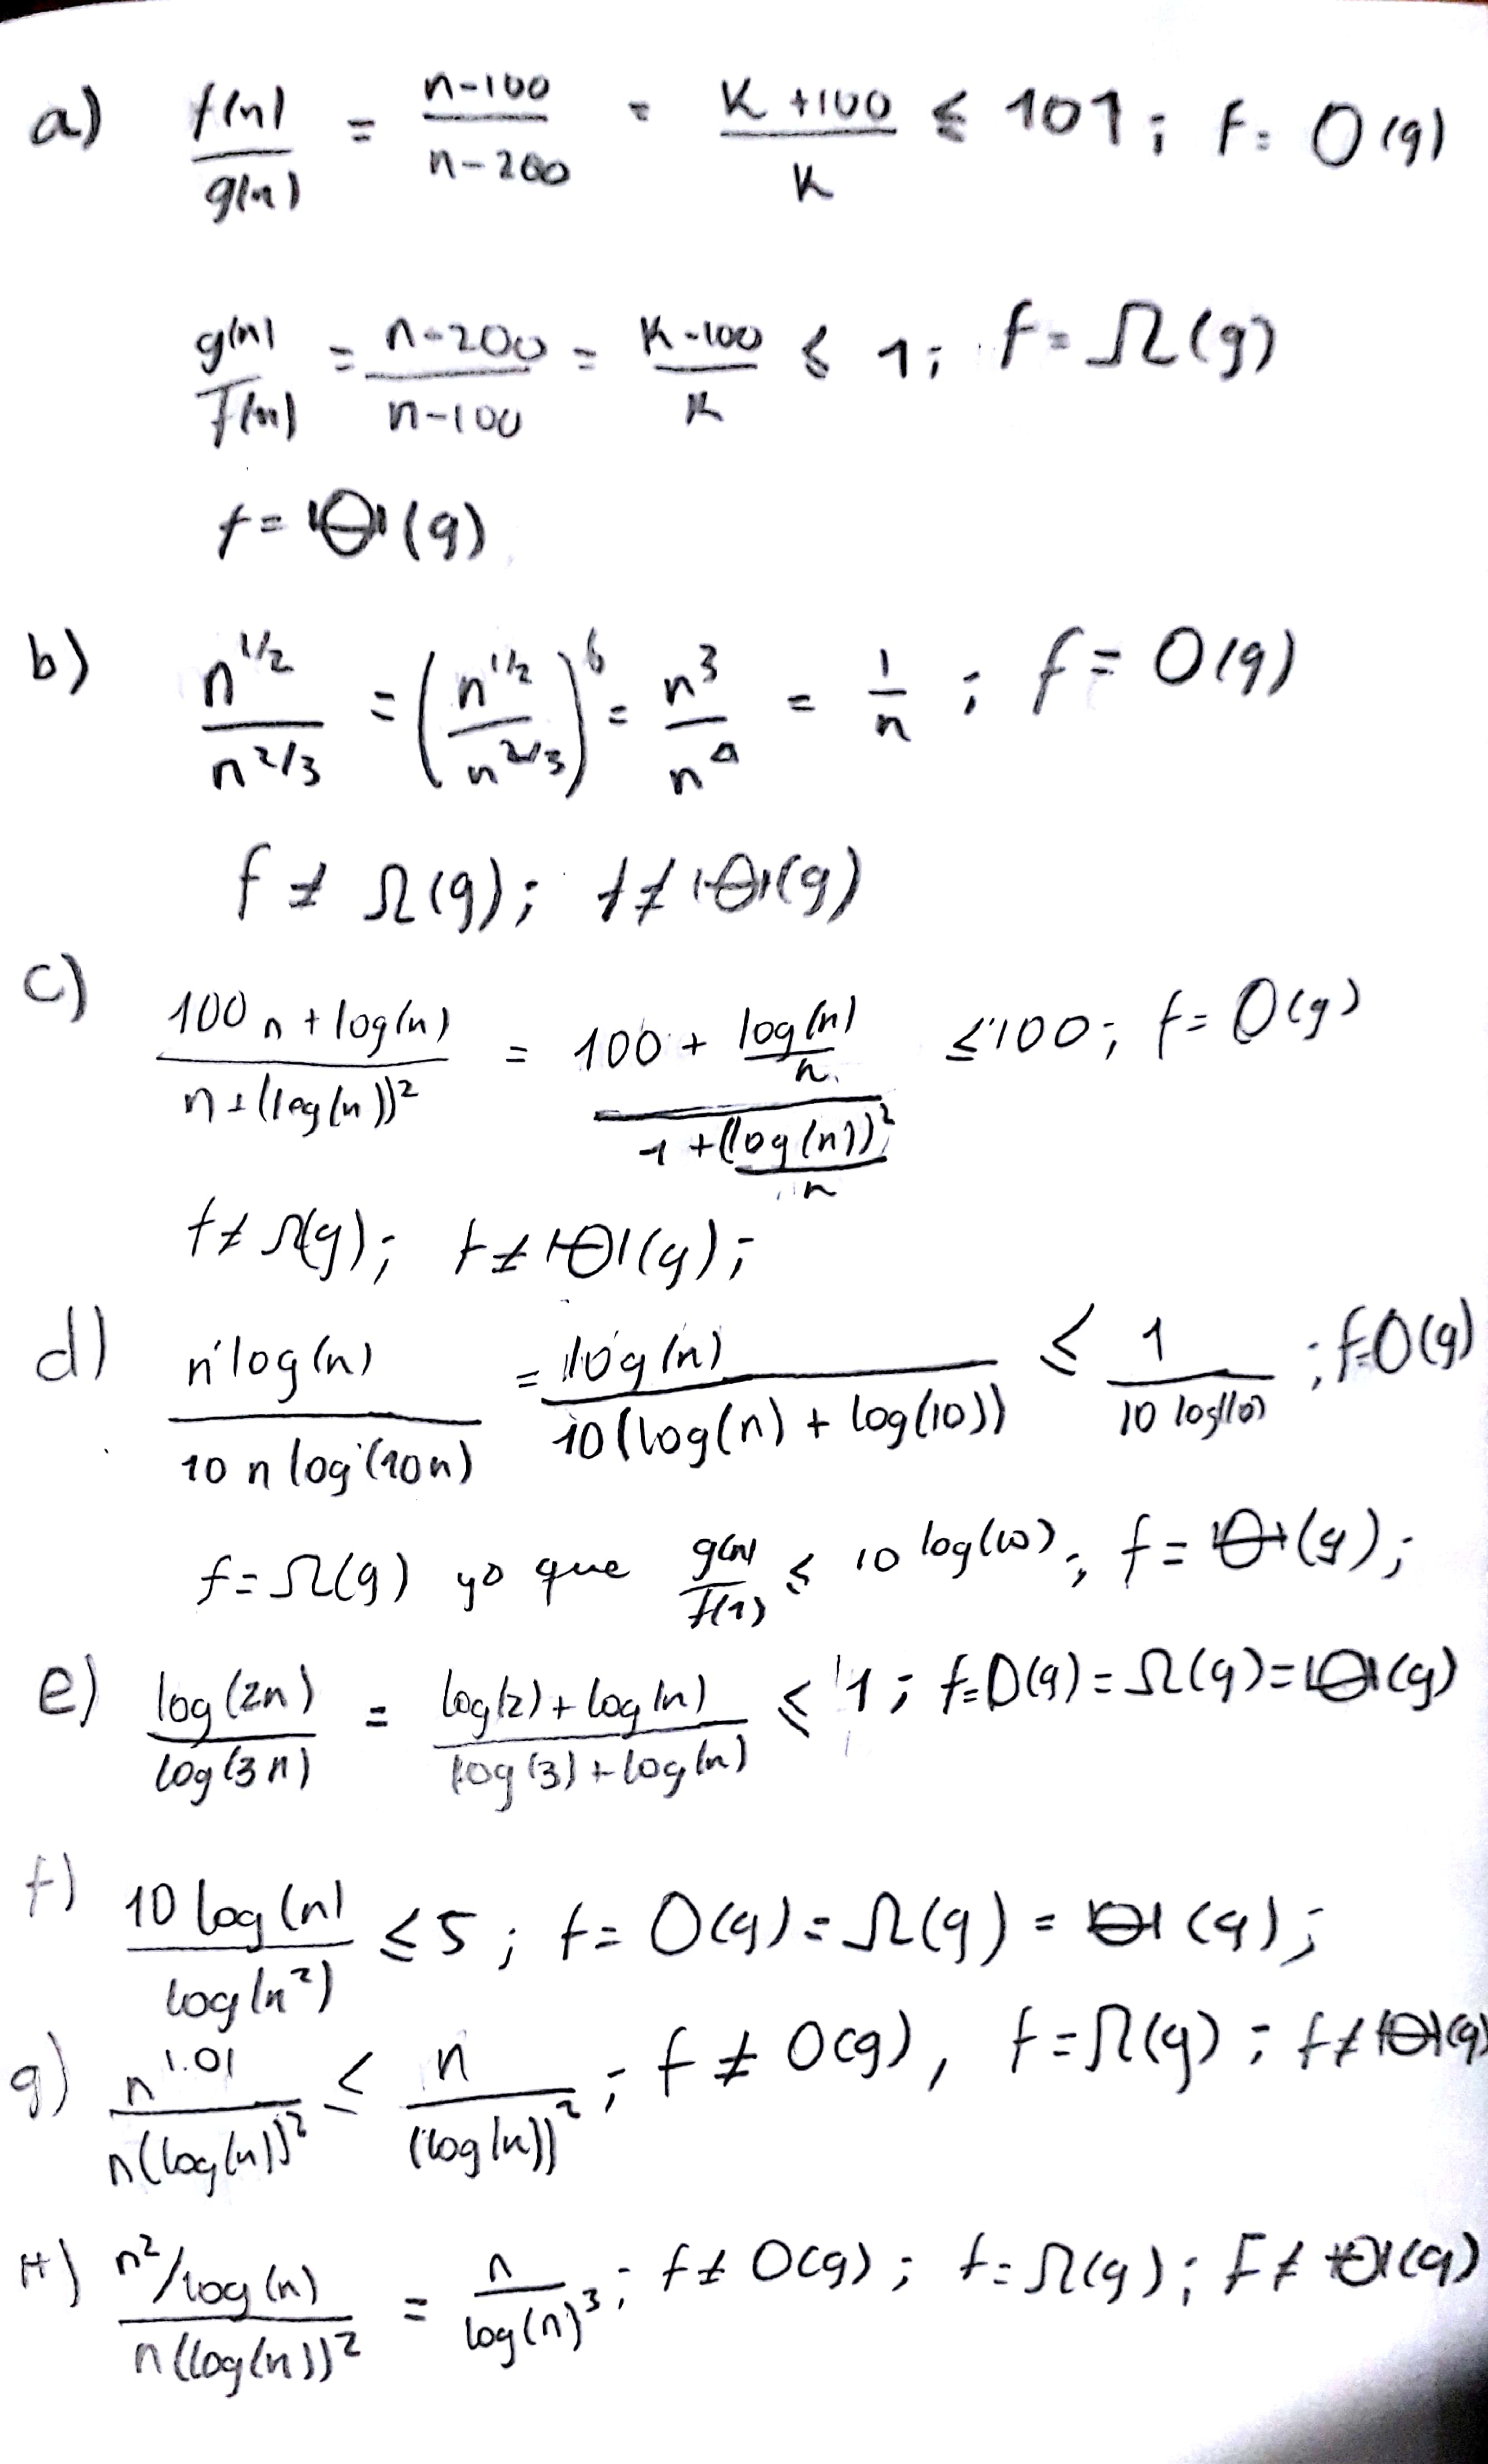
\includegraphics[width=\textwidth]{./img/DVP1}
  \caption{Solución de problemas.}
  \label{fig:DVP1}
\end{figure}

\subsection{Exercise 0.2}
Show that, if $c$ is a positive real number, then $g(n) = 1 + c + c^2 + ... + c^n$ is:

\begin{itemize}
	\item $\Theta(1)$, if $c < 1$.
	\item $\Theta(n)$, if $c = 1$.
	\item $\Theta(c^n)$, if $c > 1$.
\end{itemize}

The moral: in big-$\Theta$ terms , the sum of a geometric series is simply the first term if the series is strictly decreasing, the last term if the series is strictly increasing, or the number of terms if the series is unchanging.

\subsubsection{$c < 1$}
Las series geométricas, infinitas, convergen a una constante cuando la base de cada término, en esta caso $c$, es menor que 1. Si así lo hacen las series infinitas, con mas veras lo hará una serie geométrica finita.

\subsubsection{$c = 1$}
Cuando se reemplaza $c=1$, entonces todos los términos de la serie geométrica son $1$ y al sumarse da como resultado $n$.

\subsubsection{$c > 1$}
En el caso en el que $c > 1$, no es sencillo estimar a qué valor converge, de ser el caso, la serie geométrica, más podemos garantizar que este valor superará el mayor término, o en términos de la notación $\Theta$ sería $\Theta(c^n)$.

\section{Solving Recursions}
Solve $T(n) = 2 T(n-2) + 2$, with $n = 2k$ and for $T(0) = 0$, and $T(2) = 1$ by Recursive Substitution and the Graphical Method.

Al resolver la recursión reemplazando su definición $k$ veces, asumiendo $n = 2k$ se tiene el siguiente resultado:

$$k=0: 	T(n) = 2T(n-2) + 2 $$
$$k=1: 		 = 4T(n-4) + 2(1+2)$$
$$k=2: 		 = 8T(n-6) + 2(1+2+4)$$
$$k=3: 		 = 16T(n-8) + 2(1+2+4+8)$$
$$k: 	T(n)	 = 2^{k+1}T(n-2(k+1)) + 2^{k+2} - 1$$

Remplazando $k = n/2$ en la expresión general obtenemos:

$$T(n)	 = 2^{n/2+1}T(2) + 2^{n/2+2} - 1$$

Ya que se nos ha informado que $T(2) = 1$, se tiene la siguiente expresión para la complejidad de esta función recursiva en función de $n$.

\begin{equation}
	T(n)	 = 6(2^{n/2})- 1
\end{equation}

Por ende podemos concluir que $T(n) \in O(2^{n/2})$

\end{document}